\begin{adjustbox}{width=\textwidth}
	\begin{tikzpicture}[every node/.style={inner sep=0,outer sep=0}]
	
		\node [anchor=north east] (img1) at (-0.03\textwidth,0) {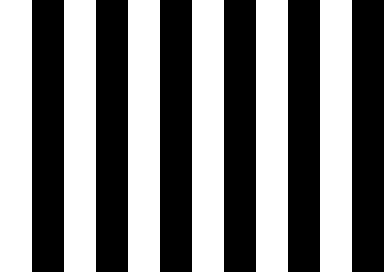
\includegraphics[frame,width=.47\textwidth]{03_sichtpruefungDurchLichtstreuung/einsatzVonMehrerenStreifenmustern/figures/rechteckStreifenmuster}};
		\node [below=0.2cm of img1] {Muster $m_1$ mit $\psi_1 = 0$};
		\node [anchor=north west] (img2) at (0.03\textwidth,0) {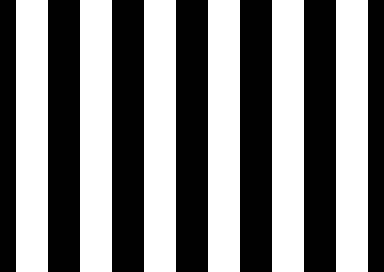
\includegraphics[frame,width=.47\textwidth]{03_sichtpruefungDurchLichtstreuung/einsatzVonMehrerenStreifenmustern/figures/rechteckStreifenmuster_shifted}};
		\node [below=0.2cm of img2] {Muster $m_2$ mit $\psi_2 = \tfrac{\pi}{2}$};
		
	\end{tikzpicture}
\end{adjustbox}
\caption[Rechteckförmiges Streifenmuster]{Streifenmuster nach Gleichung \ref{eq:rstreifenmuster}, mit $A_m = 127.5$, $N_p = 6$, $N_{shift} = 4$ und $\acrshortmath{lwidth} = 384$. Die Breite der Streifen betragen jeweils 32 Pixel.}